\documentclass[12pt,a4paper]{article}
\usepackage{ctex}
\usepackage{graphicx}
\usepackage{geometry}
\usepackage{array}
\usepackage{setspace}
\usepackage{xeCJK}
\usepackage{indentfirst}
\usepackage{amsmath}
\usepackage{float}
\usepackage{subfigure}
\usepackage{booktabs}
\usepackage{multirow}
\usepackage{caption}

% 设置页边距
\geometry{left=2.5cm,right=2.5cm,top=2.5cm,bottom=2.5cm}

% 设置行距
\linespread{1.0}

% 取消首行缩进
\setlength{\parindent}{0em}

% 设置默认字体为宋体小四
\setCJKmainfont[BoldFont=SimHei]{SimSun}
\zihao{-4}

\begin{document}

% 页眉部分
\begin{center}
  \begin{tabular}{p{0.3\textwidth}p{0.7\textwidth}}
    
\includegraphics[width=0.3\textwidth]{assets/scut_logo.png} &
    \zihao{3}\songti\textbf{大学物理实验（一）实验报告}
  \end{tabular}
\end{center}

% 标题
\begin{center}
  {\zihao{-3}\songti\textbf{葡萄糖溶液旋光率测量}}
\end{center}

\vspace{0.8cm}

% 学生信息表格（改为下划线样式）
\noindent \begin{tabular}{@{}llll}
24级\underline{\makebox[3cm][c]{x}} 班 & 
姓名\underline{\makebox[3cm][c]{Pinco Li}} & 
小组序号\underline{\makebox[3cm][c]{x}} \\[2ex]
\end{tabular}

\noindent \begin{tabular}{@{}llll}
实验日期 2025 年\underline{\makebox[1cm][c]{3}} 月 \underline{\makebox[1cm][c]{21}} 日 
& 第 4 周 
& 星期\underline{\makebox[2cm][c]{五}} 
& 指导老师\underline{\makebox[2cm][c]{x}} \\[2ex]
\end{tabular}

\noindent 同组同学\underline{\makebox[5cm][c]{x}}

\vspace{0.8cm}

% 实验目的部分标题
\textbf{一、实验目的}

a. 学习组装和使用旋光仪。

b. 深入理解光的偏振和物质的旋光性质。

c. 了解测定葡萄糖溶液旋光率和浓度的方法。

\vspace{0.5cm}
\textbf{二、实验仪器}

\textbf{1. OEX-PSP偏振光旋光测试仪}

完整套装包括半导体激光器、导轨、带转盘的起偏器、光强检测器、样品管支架和调节装置。如图1所示
\begin{figure}[H]
    \begin{minipage}[t]{0.5\linewidth}
        \centering
        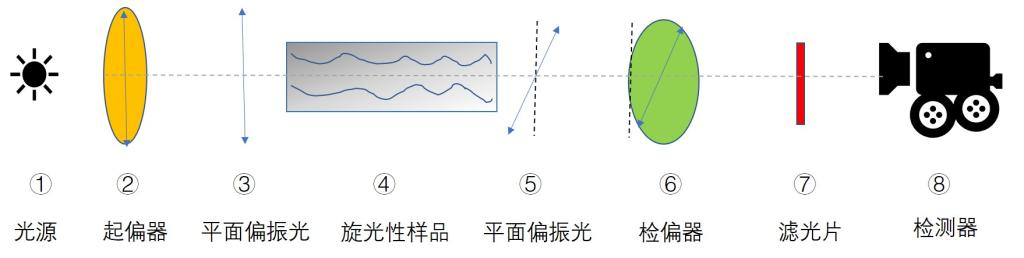
\includegraphics[clip,scale=0.1]{assets/fig1.jpg}
        \caption{OEX-PSP偏振光旋光测试仪}
        \label{figure.1}
    \end{minipage}
    \begin{minipage}[t]{0.5\linewidth}
        \centering
        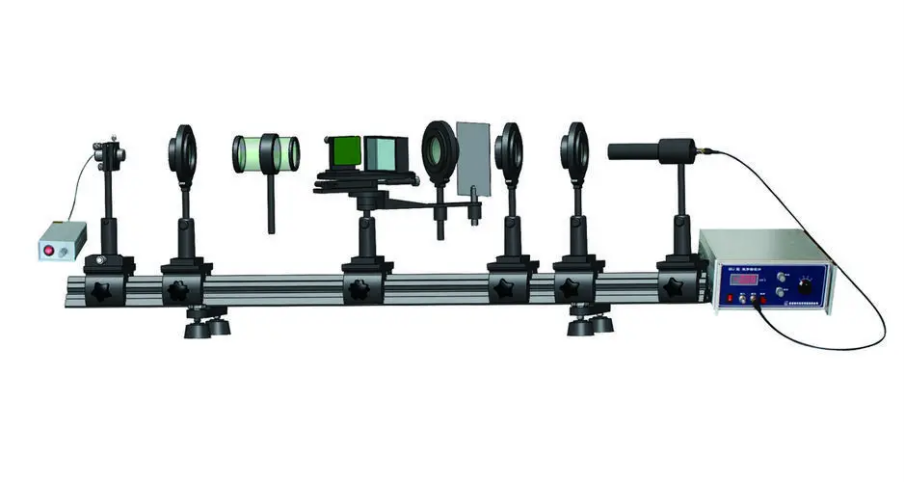
\includegraphics[clip,scale=0.8,trim={0 30 0 0}]{assets/fig2.png}
        \caption{物理演示图}
        \label{figure.2}
    \end{minipage}
\end{figure}

\textbf{2. 样品管}

含0.25g/ml质量浓度葡萄糖溶液的样品管。位于偏振片和检测器之间，用于偏转激光以检测旋光率。使用时需确保样品管与前后镜片处于相同高度和水平面。
\begin{figure}[H]
    \centering
    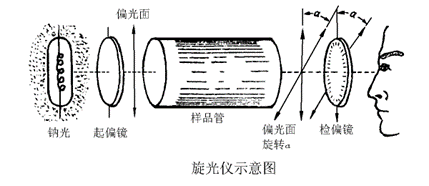
\includegraphics[clip,scale=1,trim={0 22 0 0}]{assets/fig3.png}
    \caption{实验仪器各部分详细说明}
    \label{figure.3}
\end{figure}

\vspace{0.5cm}
\textbf{三、实验原理}

许多有机化合物，如石油和葡萄糖，由于分子结构的不对称性而具有旋光特性。这些物质在所有状态下都存在旋光性，包括这些物质的溶液。一些矿物质（如石英、菊石等）也具有旋光特性，这是由于它们的晶体结构导致的，因此当晶体形式消失时，旋光特性也会消失。

\textbf{1. 光的偏振性}

光是电磁波，由于电磁波对物质的作用主要是电场，光学中将电场强度E称为光矢量。在垂直于光波传播方向的平面内，光矢量可能有不同的振动方向，光矢量保持在某一确定振动方向的状态通常称为偏振状态。如果光在传播过程中，光矢量保持固定平面振动，这种振动状态称为平面振动状态，该平面称为振动面（见图4）。此时光矢量在垂直于传播方向的平面内的投影是一条直线，因此也称为线偏振状态。如果光矢量围绕传播方向旋转，其端点描绘出一个圆的轨迹，这种偏振状态称为圆偏振状态。如果光矢量的端点沿椭圆旋转，则变成椭圆偏振状态。（见图5）
\begin{figure}[H]
    \begin{minipage}[t]{0.5\linewidth}
        \centering
        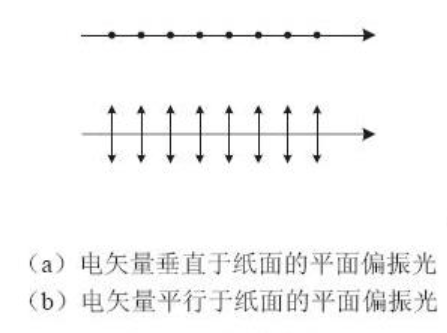
\includegraphics[clip,scale=1,trim={0 60 0 0}]{assets/fig4.png}
        \caption{平面偏振光}
        \label{figure.4}
    \end{minipage}
    \begin{minipage}[t]{0.5\linewidth}
        \centering
        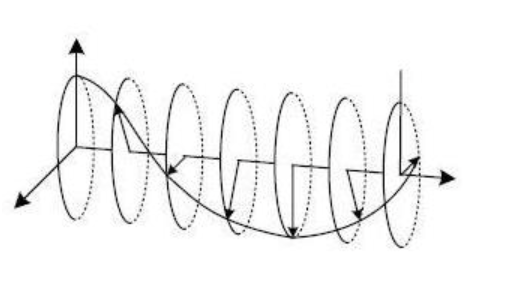
\includegraphics[clip,scale=0.8]{assets/fig5.png}
        \caption{椭圆偏振光}
        \label{figure.5}
    \end{minipage}
\end{figure}

\textbf{2. 偏振器}

虽然普通光源发出的是自然光，但自然界中存在各种偏振光。广泛使用的偏振光装置是人工偏振器，它利用二色性获得偏振光（某些各向同性介质，在某种作用下，会表现出各向异性，能强烈吸收入射光矢量在某一方向的分量并传递其垂直分量，从而将入射自然光变为偏振光，具有这种性质的介质称为二色性）。偏振装置可用于将自然光变为平面偏振光——偏振，或识别线偏振光、自然光和部分偏振光——偏振检测。用于偏振的偏振器称为起偏器，用于偏振检测的偏振装置称为检偏器。实际上，起偏器和检偏器是通用的。

\textbf{3. 旋光率}

\textbf{(1) 关于旋光率$\varphi$}

当偏振光通过这些物质时，振动面在光传播方向上旋转一个角度$\varphi$，这种现象称为旋光。

\textbf{研究表明：}

a. 对于具有旋转性质的固体物质，当偏振光通过它时，偏振平面的旋转角$\varphi$与光通过固体物质的厚度$l$成正比，即：
\begin{eqnarray}
\varphi =\alpha l 
\end{eqnarray}

b. 对于具有旋转性质的液体，当偏振光通过它时，偏振平面的旋转角$\varphi$与光通过溶液的厚度$l$和溶液的浓度$c$成正比，即：
\begin{eqnarray}
\varphi =\alpha lc
\end{eqnarray}

$\varphi$称为物质的旋光指数，与入射光波的波长和旋转物质有关。不同波长的线偏振光通过一定长度的旋光材料时，振动平面的旋转角度不同，这种现象称为旋光色散。$\varphi$也与温度有关，但影响不大。对于大多数物质，温度每升高$1^\circ C$，旋光率减小几千分之一度。

\textbf{(2) 关于左旋右旋}

旋光物质有左旋和右旋之分。当实验者面向光源观察时，振动面顺时针旋转的物质称为右旋物质，反之则为左旋物质。
\begin{figure}[H]
    \centering
    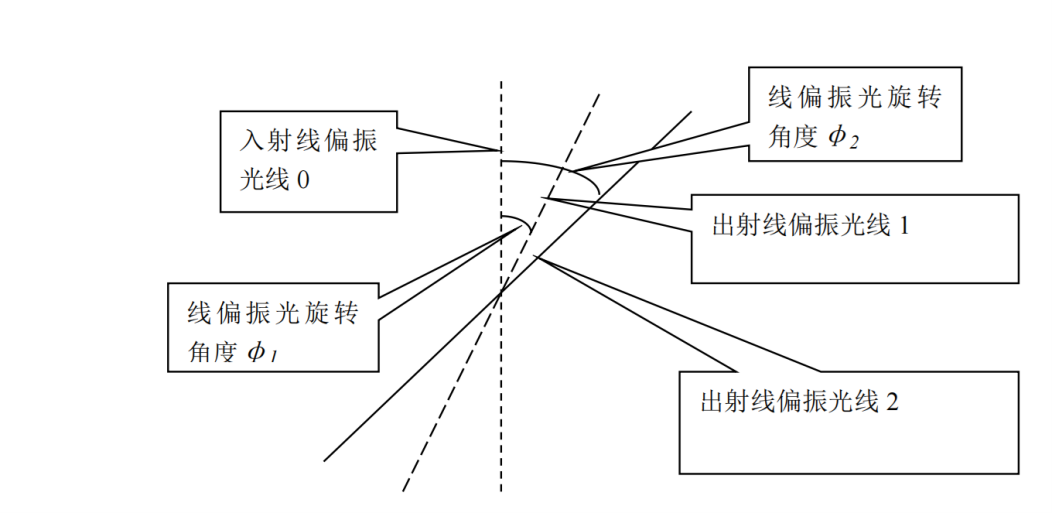
\includegraphics[clip,scale=0.5,trim={30 0 0 20}]{assets/fig8.png}
    \caption{右旋转示意图}
    \label{figure.7}
\end{figure}

如上图所示：一个简单的判断方法是选择$l_{1}$和$l_{2}$作为质数，$l_{1} > l_{2}$且差值不大；如果测得$\theta _{2} > \theta _{1}$，则可以判断该物质为右旋光物质，反之亦然。

\vspace{0.5cm}
\textbf{四、实验内容与步骤}

\textbf{使用偏振光旋光测试仪测量葡萄糖溶液的旋光率和浓度}

\textbf{(1) 偏振光旋光仪的组装}

A. 将半导体激光器、偏转器、样品管支架和光强检测器安装并固定到光学工具支架上，调整同轴轮廓使激光器发出的激光垂直通过偏转器和光强检测器的中心。

B. 调整偏振器刻度盘使输出的偏振光最强，并将偏振器固定在导轨滑块上，使偏振器和起偏器平行且在相同高度上同轴。调整偏振器刻度盘使从偏振器输出的光最强，且偏振器的偏振方向垂直于起偏器的偏振方向，并记录此时$P_{2}$的角度值${\theta}'$。旋转$P_{2}$ $360^\circ$并观察旋转过程中光强的变化。
\begin{figure}[H]
    \centering
    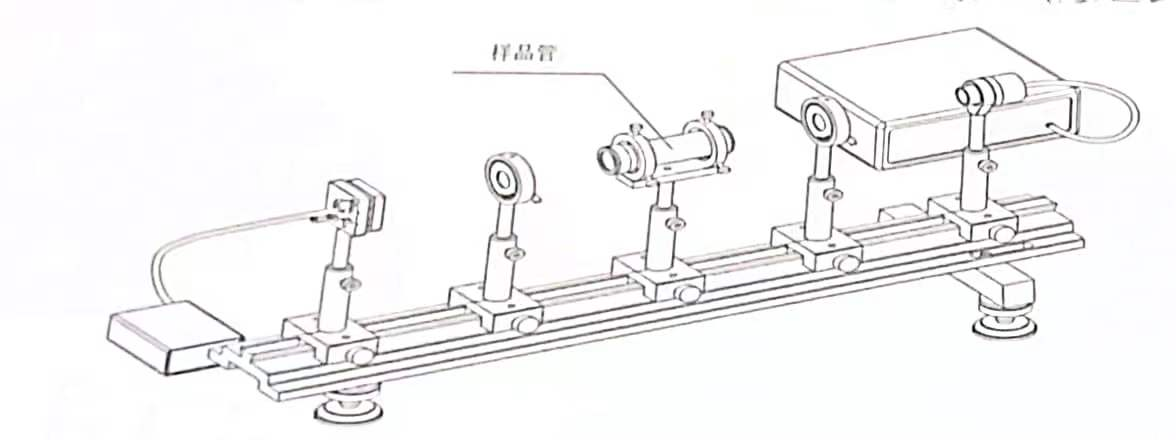
\includegraphics[clip,scale=0.2,trim={0 0 0 10}]{assets/fig10.jpg}
    \caption{操作演示图}
    \label{figure.9}
\end{figure}

\textbf{(2) 葡萄糖溶液旋光率的测量}

A. 将装有纯水的样品管放在支架上，用一张白纸观察入射到样品管和出样品管的光点是否形状相同，以检查玻璃样品管是否与激光束在相同高度上同轴。如果不同轴，调整样品管支架下的调节螺丝实现同轴。

B. 观察纯水中的旋光现象。调整检测器刻度盘使输出光强最小，记录此时$P_{2}$的角度值$\theta _{0}$，并比较$\theta _{0}$与${\theta}'$。读取一次$\theta _{0}$角度后，向一个方向旋转$P_{2}$ $360^\circ$并再次读取，共5次。

C. 将装有0.25g/ml质量浓度葡萄糖溶液的样品管放在样品管支架上。此时可以观察到通过检测器的光强不是最小值，必须旋转到某个$\theta _{i}$角度，光强检测器才显示最小值，由此测量样品为葡萄糖溶液时$P_{2}$对应的角度$\theta _{i}$（共5次）。$\theta _{i}$与$\theta _{0}$之间的差值是葡萄糖溶液的旋光度。

D. 用游标卡尺测量样品管长度L（取5个管子各测量一次）和环境温度t（实验前、中、后各一次）。

E. 使用差值法，求出物质的旋光率$\left [ \alpha  \right ] _{L}^{t}$并求旋光率的不确定度。
\begin{eqnarray} 
\theta = \left [ \alpha  \right ] _{L}^{t} lc \Longleftrightarrow \left [ \alpha  \right ] _{L}^{t}=\frac{\theta}{lc} 
\end{eqnarray}

\vspace{0.5cm}
\textbf{五、数据处理}

\textbf{葡萄糖溶液的旋光测量}

我们使用浓度为0.25g/ml，长度为15.0cm的葡萄糖溶液样品管进行测量。测量得到的放管前后角度变化如下表所示：

\begin{center}
    \begin{tabular}{ccccc}
        \toprule
        测量次数 & \multicolumn{2}{c}{角度读数} & \multicolumn{2}{c}{差值} \\
        \cmidrule(lr){2-3} \cmidrule(lr){4-5}
        & 放管前 & 放管后 & 角度差 & 平均值 \\
        \midrule
        第1次 & $90^\circ$ & $102^\circ8'$ & $12^\circ8'$ & \multirow{5}{*}{$11^\circ35'$} \\
        第2次 & $90^\circ$ & $100^\circ20'$ & $10^\circ20'$ & \\
        第3次 & $90^\circ$ & $101^\circ28'$ & $11^\circ28'$ & \\
        第4次 & $90^\circ$ & $102^\circ16'$ & $12^\circ16'$ & \\
        第5次 & $90^\circ$ & $101^\circ44'$ & $11^\circ44'$ & \\
        \bottomrule
    \end{tabular}
\end{center}

\textbf{(1) 原始数据转换为十进制度数}

为了便于进行格拉布斯检验和不确定度分析，首先将角度分数制数据转换为十进制度数：

\begin{center}
    \begin{tabular}{ccc}
        \toprule
        测量次数 & 原始数据 & 十进制度数 \\
        \midrule
        第1次 & $12^\circ8'$ & $12.133^\circ$ \\
        第2次 & $10^\circ20'$ & $10.333^\circ$ \\
        第3次 & $11^\circ28'$ & $11.467^\circ$ \\
        第4次 & $12^\circ16'$ & $12.267^\circ$ \\
        第5次 & $11^\circ44'$ & $11.733^\circ$ \\
        \bottomrule
    \end{tabular}
\end{center}

\textbf{(2) 格拉布斯检验}

使用格拉布斯检验判断是否存在异常值。计算平均值$\overline{x}$和标准偏差$s$：
\begin{eqnarray}
\overline{x} &=& \frac{1}{5}(12.133^\circ + 10.333^\circ + 11.467^\circ + 12.267^\circ + 11.733^\circ) = 11.587^\circ \\
s &=& \sqrt{\frac{\sum_{i=1}^{5}(x_i - \overline{x})^2}{5-1}} = 0.735^\circ
\end{eqnarray}

计算每个数据点的格拉布斯统计量$G_i = \frac{|x_i - \overline{x}|}{s}$：

\begin{center}
    \begin{tabular}{cccc}
        \toprule
        测量次数 & 数据值 & $|x_i - \overline{x}|$ & $G_i$ \\
        \midrule
        第1次 & $12.133^\circ$ & $0.546^\circ$ & 0.744 \\
        第2次 & $10.333^\circ$ & $1.254^\circ$ & 1.707 \\
        第3次 & $11.467^\circ$ & $0.120^\circ$ & 0.163 \\
        第4次 & $12.267^\circ$ & $0.680^\circ$ & 0.926 \\
        第5次 & $11.733^\circ$ & $0.146^\circ$ & 0.199 \\
        \bottomrule
    \end{tabular}
\end{center}

对于样本量$n=5$，99\%置信度下为1.749。

检验结果：第2次测量值的$G_2 = 1.707 < 1.749$，在99\%置信度下不是异常值。

\textbf{(3) 不确定度分析}

平均值：$\overline{x} = 11.587^\circ$

A类标准不确定度：$u_A = \frac{s}{\sqrt{n}} = \frac{0.735^\circ}{\sqrt{5}} = 0.329^\circ$

相对标准不确定度：$\frac{u_A}{\overline{x}} \times 100\% = 2.84\%$

扩展不确定度($k=2.58$)：$U = 2.58 \times u_A = 0.849^\circ$

最终旋光角测量结果为$(11.587 \pm 0.849)^\circ$，置信水平99\%。

使用该旋光角，计算葡萄糖溶液的旋光率：

\begin{eqnarray}
    [\alpha]_L^t = \frac{\theta}{lc} = \frac{11.587^\circ}{15.0 \times 0.25} = \frac{11.587^\circ}{3.75} = 3.09^\circ \cdot \text{cm}^{-1} \cdot \text{(g/ml)}^{-1}
\end{eqnarray}

转换为常用单位：
\begin{eqnarray}
    [\alpha]_L^t = 30.9^\circ \cdot \text{dm}^{-1} \cdot \text{(g/ml)}^{-1} \pm 2.3^\circ \cdot \text{dm}^{-1} \cdot \text{(g/ml)}^{-1}
\end{eqnarray}

\vspace{0.5cm}

\textbf{六、结论和分析}

\textbf{1. 实验结论}

A. 葡萄糖溶液旋光率测量：我们测得0.25g/ml浓度、15.0cm长度的葡萄糖溶液的平均旋光角为$(11.587 \pm 0.849)^\circ$（置信水平99\%，剔除异常值后）。计算得到比旋光度约为$(30.9 \pm 2.3)^\circ \cdot \text{dm}^{-1} \cdot \text{(g/ml)}^{-1}$。

B. 从旋光角度的变化可以判断葡萄糖是右旋物质，这与已知的葡萄糖性质相符。

\textbf{2. 实验误差分析}

A. 光电流计误差：实验中，光电流计读数不稳定，导致读数困难。

B. 设备误差：激光源无法长时间保持稳定的光源强度，且偏转器和检偏器无法形成完全平行的关系，导致测量中存在一定误差。

C. 环境光误差：尽管实验过程中已经尽量保持环境黑暗，但自然光的存在依然会导致仪器指示与实际激光产生的光强之间存在偏差。

D. 温度影响：实验过程中温度波动会对旋光率测量产生影响。

\textbf{七. 实验感想与改进}

A. 使用更稳定的光源和更精确的测量设备，减少系统误差。

B. 在暗室中进行实验，减少环境光干扰。

C. 增加测量次数至少7-10次，减少随机误差影响，便于更可靠地识别和处理异常值。

D. 控制实验环境温度，减少温度变化对旋光率的影响。

E. 使用多种浓度的样品进行测量，验证旋光角与浓度的线性关系。

F. 使用更高精度的角度读数装置，减少读数误差。

G. 对于数据处理，应用格拉布斯检验等统计方法对测量结果进行筛选，提高数据可靠性。

\end{document}
